% English manuscript (measurement study). Class: Elsevier CAS double column, as in the previous manuscript.
% Build: pdflatex main && bibtex main && pdflatex main && pdflatex main  (needs cas-dc.cls, cas-common.sty, references.bib in this folder).
% Every red "[NO DATA YET: ...]" marks a number or sentence that must come from a measurement listed in TODO.md; none is estimated.
\documentclass[a4paper,fleqn]{cas-dc}

\usepackage[utf8]{inputenc}
\usepackage[T1]{fontenc}
\usepackage[numbers,sort&compress]{natbib}
\usepackage{amsmath,amssymb}
\usepackage{booktabs}
\usepackage{tabularx}
\usepackage{array}
\usepackage{enumitem}
\usepackage{microtype}
\usepackage{hyperref}
\usepackage{xcolor}
\usepackage{graphicx}
\graphicspath{{figures/}{./}}
\usepackage{tikz}
\usetikzlibrary{arrows.meta,positioning}

% Placeholder for results that have not been measured yet. Search the source for "NO DATA YET" before submission.
\newcommand{\nodata}[1]{\textcolor{red}{[NO DATA YET: #1]}}
\newcommand{\figtodo}[2]{\begin{center}\fbox{\parbox{0.92\linewidth}{\centering\textcolor{red}{[FIGURE PENDING: #1]}\\ \footnotesize #2}}\end{center}}
\newcommand{\Ntau}{N_{\tau}}

\begin{document}
\let\WriteBookmarks\relax
\def\floatpagepagefraction{1}
\def\textpagefraction{.001}
\shorttitle{Candidate count and detector latency}
\shortauthors{Pham and Mai}
\title[mode=title]{Does the Number of Pre-NMS Candidates Predict Detector Latency? A Pinned-Core Measurement Study with a Patch-Optimization Case Study}
\author[1]{Pham Tuan Anh}
\ead{anh25807700004@hutech.edu.vn}
\author[1]{Mai Quoc Bao}
\ead{bao2580770008@hutech.edu.vn}
\cortext[cor1]{Corresponding author: Dinh Phuong Nam. Email: dp.nam@hutech.edu.vn.}
\nonumnote{Supervisor: Dinh Phuong Nam, Ho Chi Minh City University of Technology (HUTECH). Email: dp.nam@hutech.edu.vn.}
\affiliation[1]{organization={Ho Chi Minh City University of Technology (HUTECH)},
city={Ho Chi Minh City},country={Vietnam}}

\begin{abstract}
Latency-oriented adversarial inputs for object detectors commonly use the number of candidate boxes that enter non-maximum suppression (NMS), $\Ntau$, as the quantity to maximize, on the assumption that more candidates mean a slower pipeline. We ask whether $\Ntau$ is in fact a reliable predictor of latency. We build a measurement protocol with verified core pinning, per-stage timing, and an A/A calibration that yields the minimum detectable effect (MDE) of every comparison, and we apply it on a pinned laptop CPU; an Arm smartphone SoC was also prepared but could not be pinned. A positive control injects $10^2$ to $10^4$ synthetic candidates into the same pipeline and shows how NMS latency depends on $\Ntau$, on the NMS implementation, and on box geometry. We then use a genetic-algorithm patch optimizer as a case study: patches are optimized on 100 images at 320 and 640 pixels and at two score thresholds, re-measured under the pinned protocol, and used to test how well an $\Ntau$-only predictor calibrated on synthetic injections predicts the latency of real candidate sets. Injecting $10^2$ to $10^4$ candidates raises NMS latency 4- to 1360-fold depending on implementation and geometry. Patches from the genetic optimizer did not raise $\Ntau$ detectably at 320 px, and a gradient baseline that raised $\Ntau$ 2.3-fold left end-to-end time unchanged within the 0.55\% MDE (ratio 1.006, 95\% interval 0.997 to 1.015). An $\Ntau$-only predictor errs by about 5\% for one NMS implementation and by a factor of 4 for another. The smartphone could not be pinned under load, so no Arm result is reported.
\end{abstract}

\begin{keywords}
object detection \sep non-maximum suppression \sep latency measurement \sep adversarial patch \sep measurement methodology \sep Arm
\end{keywords}
\maketitle

\section{Introduction}
Object detectors that rely on NMS spend part of every frame suppressing overlapping candidate boxes. Because the cost of greedy NMS depends on how many candidates survive the score threshold, a line of work crafts inputs that raise this number in order to slow detection down \cite{phantom2023,overload2024}, extending the broader idea of energy-latency attacks on neural networks \cite{shumailov2021sponge}. In these works the candidate count $\Ntau$ plays two roles at once: it is the quantity the optimizer maximizes, and it is the explanation offered for the resulting slowdown. The second role is an empirical claim, and it can fail. The cost of NMS also depends on the implementation and on how the candidate boxes overlap, and NMS is only one stage of a pipeline that also contains the network forward pass.

This paper treats the relation between $\Ntau$ and latency as a measurement problem and asks four questions.
\begin{description}[leftmargin=2.2em,labelwidth=2em,itemsep=1pt]
\item[Q1] Under a calibrated protocol, how does NMS latency depend on $\Ntau$ when the candidates are controlled, over $10^2$ to $10^4$ candidates?
\item[Q2] At equal $\Ntau$, how much do NMS implementation and box geometry change that latency?
\item[Q3] For candidate sets produced by optimized patches on real images, how much do $\Ntau$, NMS latency, and end-to-end latency change relative to clean images, compared with the noise floor of the protocol?
\item[Q4] How well does an $\Ntau$-only predictor, calibrated on synthetic injections, predict the NMS latency of those real candidate sets?
\end{description}

\paragraph{Contributions.}
(i) A measurement protocol for pipeline latency with core pinning verified under load, stage-wise timing, and an A/A calibration that reports the MDE of every comparison. (ii) A positive control that injects synthetic candidates at the decoded-output boundary of a real pipeline and maps latency as a function of $\Ntau$, implementation, geometry, and top-$k$ cap, on a pinned laptop CPU (the Arm smartphone could not be pinned under load). (iii) A case study of a published-style genetic patch optimizer scaled to 100 optimization images, 640-pixel inputs, and a 0.25 score threshold, with comparison to random-search, placement, and gradient baselines. (iv) A direct test of the $\Ntau$ proxy: prediction error of an $\Ntau$-only model on held-out real candidate sets. The protocol, the hypotheses, and the endpoints were fixed in a public repository before the corresponding measurements were taken.

\paragraph{Organization.}
Section~2 positions the study against prior work, Section~3 formalizes $\Ntau$ and the quantities compared, Section~4 describes the measurement protocol, the positive-control design, the case-study optimizer, and the preregistration record, Section~5 reports the experiments, Section~6 discusses what the results do and do not show, and Section~7 collects the threats to validity.

\section{Related Work}
\paragraph{Energy-latency and sponge attacks.}
Sponge examples increase the energy or latency of a network through crafted inputs \cite{shumailov2021sponge}. For object detection, Phantom Sponges craft a universal perturbation that inflates the number of boxes entering NMS \cite{phantom2023}, Overload optimizes inputs with a spatial-attention weighting and evaluates on edge hardware \cite{overload2024}, and SlowTrack carries latency attacks to the camera-based perception chain of driving systems \cite{slowtrack2024}. Related efficiency attacks target captioning models \cite{nicgslowdown2022} and inference hardware faults \cite{bitflip2025}, and defences train detectors to resist latency attacks \cite{underload2025}. The detector-level works use the number of candidates, or a close surrogate, as the optimization target; they report latency increases on their chosen models and devices. We do not propose a stronger attack. We test the relation that the optimization target relies on.

\paragraph{Practicality of NMS latency attacks.}
EVADE examines whether NMS latency attacks matter in realistic deployments, considering hardware, model formats, quantization, and downstream latency requirements \cite{evade2025}. Our study is complementary in three ways. First, it isolates the candidate-to-latency relation by injecting controlled candidate sets, which provides a positive control that attack-generated inputs cannot, because attack inputs change the image and the candidates together. Second, it quantifies the noise floor of each comparison with an A/A design and reports effects relative to the MDE rather than as bare ratios. Third, it tests an $\Ntau$-only predictor on real candidate sets and reports where the predictor holds and where it fails. EVADE addresses the question of whether an attack is practical; we address the question of what the optimized quantity can and cannot predict.

\paragraph{Adversarial patches and robust optimization.}
Adversarial patches are local, image-agnostic perturbations \cite{brown2017patch}, and expectation over transformation (EOT) optimizes them over random image transformations so that they survive resizing, rotation, and photometric change \cite{athalye2018eot}; patches have been applied against person detectors \cite{thys2019fooling}. Our case-study optimizer uses a software EOT with rotation, color jitter, blur, and noise, and inserts the patch digitally.

\paragraph{Query-based black-box optimization.}
Query-efficient black-box attacks estimate or search over inputs using only model outputs \cite{ilyas2018blackbox}. The case-study optimizer is score-based in the same sense: its fitness uses the detector's pre-NMS class scores and no gradients. It is not a query-limited remote attack, because it reads pre-NMS scores that a deployed service would not return, and we state this access assumption where the method is described.

\paragraph{Latency measurement and noise.}
Wall-clock latency on a general-purpose operating system is affected by frequency scaling, thermal state, background activity, and the scheduler. Reports of an attack-induced slowdown are only interpretable if the run-to-run variation of the unattacked system is known, and it is not always stated. We therefore borrow a standard device from experimental practice: an A/A comparison, in which both arms are the same condition, gives the variance of the paired difference and hence the smallest effect that the design could have detected. Every ratio in this paper is read against that value.

\paragraph{Detectors without NMS.}
NMS is a feature of dense, anchor-based detectors. Set-prediction detectors such as DETR remove it from the architecture \cite{carion2020detr}. Latency attacks that target NMS cannot apply to these designs by construction, so the question studied here concerns a particular, widely deployed family: YOLO-style one-stage detectors followed by greedy suppression \cite{redmon2016yolo,neubeck2006nms}.

\begin{table*}[t]
\centering\small
\caption{Positioning against closely related work. The first five rows summarize what each work reports at the level of detail relevant here; the last row describes this study.}
\label{tab:related}
\begin{tabularx}{\textwidth}{@{}p{2.6cm}p{3.6cm}p{3.6cm}X@{}}
\toprule
Work & Target & Optimized or studied quantity & Role of the candidate count \\
\midrule
Sponge Examples \cite{shumailov2021sponge} & Neural networks (several modalities) & Energy and latency of inference & Not specific to NMS \\
Phantom Sponges \cite{phantom2023} & Object detectors with NMS & Boxes surviving the threshold, via a universal perturbation & Optimized quantity and explanation of slowdown \\
Overload \cite{overload2024} & Object detectors, edge hardware & Detector latency, with a spatial-attention weighting & Optimized quantity and explanation of slowdown \\
SlowTrack \cite{slowtrack2024} & Camera-based perception chain for driving & System-level latency over a multi-frame chain & Not examined here (chain-level work) \\
EVADE \cite{evade2025} & NMS latency attacks, realistic deployments & Practicality across hardware, formats, quantization, latency requirements & Attack objective under evaluation \\
\textbf{This study} & YOLOv8n pipeline, laptop CPU (Arm SoC attempted) & Relation between $\Ntau$ and latency, calibrated with a positive control and an A/A noise floor & The hypothesis under test \\
\bottomrule
\end{tabularx}
\end{table*}

\section{Problem Formulation}
Let a detector produce $A$ anchors for an image $x$, with class-agnostic score $s_i(x)=\max_c p_{i,c}(x)$ for anchor $i$. The candidate count at threshold $\tau$ is
\begin{equation}
\Ntau(x)=\bigl|\{\, i : s_i(x) > \tau \,\}\bigr| .
\end{equation}
For the YOLOv8n detector used here, $A=2100$ at a $320\times320$ input and $A=8400$ at $640\times640$. The end-to-end latency decomposes into pre-processing, the network forward pass, decoding, score filtering, and NMS:
\begin{equation}
t_{\mathrm{total}} = t_{\mathrm{pre}} + t_{\mathrm{fwd}} + t_{\mathrm{dec}} + t_{\tau} + t_{\mathrm{NMS}} .
\end{equation}
Only $t_{\tau}$ and $t_{\mathrm{NMS}}$ depend directly on $\Ntau$. The proxy claim examined here is that, for a fixed pipeline, $\Ntau$ determines $t_{\mathrm{NMS}}$, and through it $t_{\mathrm{total}}$. Greedy NMS repeatedly selects the highest-scoring box and removes the boxes it overlaps, so its cost grows with the number of boxes that remain selected as well as with $\Ntau$ \cite{neubeck2006nms}; this is why box geometry is a factor under test and not a nuisance.

\paragraph{Effect sizes relative to a noise floor.}
For a comparison of two conditions with paired per-image log-ratios $d_i$ ($i=1,\dots,n$) and sample standard deviation $\hat\sigma_d$, the minimum detectable effect at significance $\alpha=0.05$ and power $0.8$ is
\begin{equation}
\mathrm{MDE}=\bigl(t_{1-\alpha/2,\,n-1}+t_{0.8,\,n-1}\bigr)\,\hat\sigma_d/\sqrt{n},
\end{equation}
reported as a percentage change in latency. An A/A experiment, in which both arms are the same condition, estimates $\hat\sigma_d$ for each device, profile, and stage. We interpret a measured ratio only against this MDE. A confidence interval that contains one is never read as equivalence.

\subsection{What the cost model predicts}
We state the expected behaviour of the NMS stage before the data, so that the measurements can contradict it. Greedy suppression selects the highest-scoring remaining box, removes every remaining box whose IoU with it exceeds the threshold, and repeats. Let $K$ be the number of boxes that are selected. A straightforward vectorized implementation performs $K$ iterations, each touching the boxes that remain, so its cost is between $O(\Ntau)$ (a few selected boxes, as in a dense cluster) and $O(\Ntau^2)$ (all boxes selected, as when boxes are disjoint). The cost therefore depends on the geometry through $K$, not on $\Ntau$ alone. Library kernels use the same algorithm in compiled code, with a much smaller per-iteration constant, and batched class-aware variants offset the boxes of each class instead of looping over classes. Two further mechanisms bound the cost in practice: a cap on the number of candidates passed to NMS (top-$k$), which fixes $\Ntau$ at most at $k$, and a time limit inside the Ultralytics post-processing. We label these expectations as follows and examine them in Section~\ref{sec:results}.
\begin{description}[leftmargin=2.2em,labelwidth=2em,itemsep=1pt]
\item[H1] For a fixed implementation, NMS latency increases with $\Ntau$ over $10^2$ to $10^4$ candidates.
\item[H2] At equal $\Ntau$, disjoint boxes cost more than overlapping boxes, and the gap is largest for a loop-based implementation.
\item[H3] A top-$k$ cap lowers the latency of every implementation when $\Ntau$ exceeds $k$.
\item[H4] Because $t_{\mathrm{NMS}}$ is one term of $t_{\mathrm{total}}$, an increase of $t_{\mathrm{NMS}}$ translates into an end-to-end increase only to the extent that $t_{\mathrm{NMS}}$ is a sizable share of $t_{\mathrm{total}}$.
\end{description}

\section{Measurement Protocol}
\subsection{Pipeline and stages}
The detector is YOLOv8n \cite{jocher2023ultralytics}, a one-stage detector of the YOLO family \cite{redmon2016yolo}, run in PyTorch \cite{paszke2019pytorch}. The pipeline resizes an RGB image directly to the detector input without letterboxing, runs the network in float32, decodes the head output, applies the score threshold $\tau$ and an optional top-$k$ cap, and runs NMS with IoU threshold 0.45 and at most 300 outputs. Each stage is timed separately with a monotonic nanosecond clock, with garbage collection disabled inside the timed region, after warm-up runs that are discarded. The end-to-end time is measured in one call and is never assembled by adding stage medians. All inputs are tensors prepared in memory, so file reading and camera capture are outside the timed region (Fig.~\ref{fig:pipeline}).


\begin{figure}[t]
\centering
\begin{tikzpicture}[node distance=3.2mm, every node/.style={font=\scriptsize}, box/.style={draw, rounded corners=1pt, minimum height=5.5mm, inner sep=2pt, align=center}]
\node[box] (a) {Resize};
\node[box, right=of a] (b) {Forward};
\node[box, right=of b] (c) {Decode};
\node[box, right=of c] (d) {$\tau$, cap};
\node[box, right=of d] (e) {NMS};
\draw[-{Stealth[length=1.6mm]}] (a)--(b);
\draw[-{Stealth[length=1.6mm]}] (b)--(c);
\draw[-{Stealth[length=1.6mm]}] (c)--(d);
\draw[-{Stealth[length=1.6mm]}] (d)--(e);
\node[box, below=5mm of c, dashed] (inj) {synthetic candidates\($N_\tau$ controlled)};
\draw[-{Stealth[length=1.6mm]}, dashed] (inj.east) -| (d.south);
\node[above=1.5mm of b, xshift=3mm] {$t_{\mathrm{fwd}}$};
\node[above=1.5mm of d, xshift=2mm] {$t_{\tau}$};
\node[above=1.5mm of e] {$t_{\mathrm{NMS}}$};
\end{tikzpicture}
\caption{Pipeline stages timed separately. The dashed path shows the injection point of the positive control: synthetic candidate sets replace the decoded output and enter the score filter, so the filter and NMS stages are measured with a controlled $N_\tau$.}
\label{fig:pipeline}
\end{figure}

\subsection{NMS implementations}
Four implementations receive identical post-threshold candidates. A pure-PyTorch loop (class-agnostic) is the implementation used by the optimization code. The torchvision \texttt{nms} routine (class-agnostic) and \texttt{batched\_nms} (class-aware) are the library kernels. The native Ultralytics post-processing, which is class-aware and has its own caps and time limit, is the default of the detector's own pipeline. On finite samples without score ties, implementations within the same class-awareness group keep identical sets of boxes; this is tested but is not claimed to hold for all ties.

\subsection{Devices, core pinning, and verification}
The laptop is an Intel Core i5-1335U (two performance cores with SMT and eight efficiency cores) under Windows. The second device is a smartphone with a Snapdragon 6 Gen 3 SoC (eight Arm cores in two clusters according to the vendor specification), running Ubuntu inside a proot environment on Android. Processes are pinned to one logical CPU per physical core. Pinning is never assumed to work: for each profile we run a matrix-multiplication load with twice as many threads as allowed CPUs and require (a) the process CPU time divided by wall time not to exceed the number of allowed CPUs, (b) at least half a core of throughput for single-core profiles, and (c) for the smartphone, that at least 99\% of sampled last-run CPU indices of all threads fall inside the allowed set. On the smartphone the clusters are identified by single-CPU speed benchmarks and the thread count reported by the framework is not trusted. A profile that fails verification is not measured.

\subsection{A/A calibration and thermal control}
Each profile measures 100 held-out images, each 20 times, with the two arms labelled A and B in interleaved ABBA/BAAB order. The per-image log-ratio of arm medians gives $\hat\sigma_d$ and the MDE. A fixed reference benchmark is run at the start of the session, before each block, and at the end, and a block is flagged when it deviates by more than 3\% from the session start. On the smartphone, measurements are taken in short bursts with rest periods, profiles are interleaved across bursts so that accumulated heat is shared, and the number of flagged blocks is reported with the results.

\subsection{Statistics}
The unit of inference is the image for A/A and dose-response analyses and the (image, patch seed) pair for patch analyses. Confidence intervals are percentile intervals from 20{,}000 bootstrap resamples with a fixed seed; for patch analyses both images and seeds are resampled (a two-level percentile bootstrap; cf.\ the cluster bootstrap of \cite{cameron2008cluster}, which is a wild cluster bootstrap-$t$ and is cited for the clustering idea only) \cite{efron1979bootstrap}. Rank correlations are Spearman correlations. Comparisons that form a family of hypothesis tests would be adjusted with Holm's procedure \cite{holm1979}; the analyses here are estimates with intervals and are not tests. Analyses defined after seeing data are labelled post hoc.

\subsection{Positive-control design}
The injection replaces the decoded detector output by a synthetic candidate set that enters the score filter and NMS stages (Fig.~\ref{fig:pipeline}). A candidate set is defined by the number of anchors $A$, the target $\Ntau$, the number of classes $n_c$ (80 or 1), and a geometry. Disjoint sets place boxes on a grid, each box covering 80\% of its cell, so that no two boxes overlap (IoU of zero) and NMS keeps all of them; this is the worst case for the greedy loop. Dense-cluster sets place boxes of about 48 px, jittered by up to 2 px, around eight centres, so that boxes within a cluster overlap with IoU above the threshold and most are removed early. Mixed sets use half of each, in random order. The $\Ntau$ active candidates have scores drawn uniformly between just above $\tau=0.01$ and one and a random class; the remaining anchors of the head receive scores below $\tau/2$, so that exactly $\Ntau$ candidates pass the filter. All draws come from a seeded generator, and each set is hashed. The grid has three parts: the head of the 320-px detector ($A=2100$; $\Ntau\in\{0,10,30,100,300,600,1000,1500,2100\}$, $n_c\in\{80,1\}$), the head of the 640-px detector ($A=8400$; $\Ntau\in\{0,100,300,1000,3000,8400\}$), and a synthetic head with $A=10{,}000$ that exceeds any real head and is used only to reach $\Ntau=10^4$ ($\Ntau\in\{100,300,1000,3000,10^4\}$). All three geometries, both cap settings (none and 300), and all four implementations are crossed with these, giving 123 measurement groups. Each group is measured 30 times after 3 discarded warm-ups; the order of implementations inside a block follows a Latin-square design, and 12 groups form a block that starts with a reference benchmark. The IoU threshold is 0.45. A separate pipeline test injects $\Ntau\in\{0,100,300,1000,2100\}$ disjoint boxes into the full pipeline of one fixed image, for the pure-PyTorch and the Ultralytics implementations, 20 repetitions each, and counts the repetitions that exceed a 100~ms reference deadline (a value chosen by the authors, not an application requirement).

\subsection{Specification of the case-study optimizer}
Table~\ref{tab:spec} lists the optimizer settings. Candidate patches are scored on a fixed training set of 100 COCO training images with a software EOT (rotation, color jitter, blur, and noise; one draw per evaluation). The budget is expressed in candidate--image forward passes: 10{,}000, 25{,}000, and 62{,}500, which correspond to 100, 250, and 625 candidate evaluations over the 100 images; the final checkpoint is the one analysed, and the earlier two are kept to show saturation. The patch location is the window of maximum Laplacian variance of each image (saliency placement), except in the placement baselines. Patches were generated on a GPU (Tesla V100) because the CPU cost of the full budget over ten seeds is prohibitive; since GPU and CPU random number generators differ, the patches are not byte-identical to what the CPU code would produce, and the hash of each saved patch is the ground truth for what was measured. The gradient baseline uses a tanh parameterization of the patch and ascends the mean over images of $\sum_i \tanh(s_i)$ with respect to the patch pixels; it needs gradients through the detector and is therefore a white-box reference.

\begin{table}[t]
\centering\small
\caption{Settings of the case-study conditions. $\tau_{\mathrm{obj}}$ is the threshold inside the optimization objective. All conditions use 100 training images, software EOT, ten seeds (0--9), and the same three budgets.}
\label{tab:spec}
\begin{tabular}{@{}llccc@{}}
\toprule
Condition & Method & Input (px) & Patch (px) & $\tau_{\mathrm{obj}}$ \\
\midrule
C1 & GA, saliency placement & 320 & 64 & 0.01 \\
C2 & GA, saliency placement & 640 & 128 & 0.01 \\
C3 & GA, saliency placement & 320 & 64 & 0.25 \\
C4 & GA, saliency placement & 640 & 64 & 0.01 \\
B1 & GA, centre placement & 320 & 64 & 0.01 \\
B2 & GA, random placement & 320 & 64 & 0.01 \\
B3 & random search, saliency & 320 & 64 & 0.01 \\
B4 & gradient ascent (tanh) & 320 & 64 & 0.01 \\
\bottomrule
\end{tabular}
\end{table}

\subsection{Preregistration and deviations}
Hypotheses, endpoints, and decision rules for each experiment were written in a preregistration file and fixed with a version-control tag before the corresponding measurement (tags for the positive control, the smartphone protocol, the patch re-measurement, and the patch generation were set together; the bridging addendum for the 640-px baseline has its own tag). Deviations from the plan are listed in Table~\ref{tab:dev} and in the repository; none changed an endpoint or a decision rule after data had been seen, except the addition of a missing control, which is itself reported as a deviation.

\begin{table}[t]
\centering\small
\caption{Deviations and negative outcomes of the study. All raw records, including the discarded ones, are kept in the repository.}
\label{tab:dev}
\begin{tabularx}{\columnwidth}{@{}lX@{}}
\toprule
Item & What happened and how it was handled \\
\midrule
Early A/A runs & Two earlier A/A attempts were invalid; they are kept but not used. The analysed A/A run is the third. \\
A/A analysis timing & The analysis script was started on a measurement that was still running; the partial summary was discarded and the analysis was repeated after the run had finished. \\
Reference drift & The A/A run had 2 of 11 drift-flagged reference points, the positive control 2 of 12, and the patch re-measurement 0 of 11; flagged blocks stay in the primary analysis. \\
Backend defect at $\Ntau=6$ & The first full patch re-measurement stopped when a candidate set with exactly six boxes was misread by the Ultralytics post-processing as an end-to-end output. The input construction was fixed, a regression test was added, and the whole re-measurement was repeated; the aborted run is kept. \\
Missing 640-px baseline & The patch re-measurement had no clean 640-px arm, so 640-px results could not be read. An addendum added the arm, with an A/A at 640 px, and was tagged before its measurement. \\
Smartphone & Core pinning could not be verified under load on either cluster of the device; no timing was taken, and no smartphone result is reported. \\
\bottomrule
\end{tabularx}
\end{table}

\section{Experiments}
\label{sec:results}
\subsection{Protocol calibration (A/A)}
Table~\ref{tab:aa} reports the MDE of each stage on the pinned laptop profile (logical CPU~2, one torch thread; effective cores 0.91 under load). The end-to-end MDE is 0.55\%, and the MDE of the NMS stages is 0.64\% (pure PyTorch) and 1.1\% (torchvision). Two of the 11 reference-benchmark points of this run exceeded the 3\% drift flag (blocks 1 and 3, largest change 26\%); excluding the two flagged blocks leaves 80 images, and the end-to-end A/A difference stays within $\pm0.5\%$ (95\% interval for the mean log ratio $-0.0038$ to $0.0046$). The A/A of the other planned profiles (laptop efficiency core, smartphone) is not available: the smartphone did not pass pin verification (Section~\ref{sec:phone}).

\begin{table}[t]
\centering\small
\caption{A/A calibration on the pinned laptop profile: minimum detectable effect (MDE, \%) and median time per stage, 100 images $\times$ 20 repetitions (2 of 11 reference points were drift-flagged; they are kept in the analysis).}
\label{tab:aa}
\begin{tabular}{@{}lcc@{}}
\toprule
Stage & MDE (\%) & Median time (ms) \
\midrule
Pre-processing & 1.0 & 5.60 \
Forward pass & 0.69 & 45.8 \
Score filter ($\tau$) & 1.0 & 0.066 \
NMS (pure PyTorch) & 0.64 & 1.14 \
NMS (torchvision) & 1.1 & 0.101 \
End to end & 0.55 & 53.5 \
\bottomrule
\end{tabular}
\end{table}

\subsection{Positive control: synthetic candidate injection}
We replace the decoded detector output with a synthetic candidate set of size $\Ntau\in\{10^2,\dots,10^4\}$ and measure the score-filter and NMS stages in isolation, for the four implementations, three box geometries, two class counts, and two cap settings. The geometries are disjoint boxes (no overlap, so NMS keeps every box), dense clusters (heavy overlap, so most boxes are removed early), and an even mixture. Candidate sets are generated deterministically from a seed and hashed. For input sizes of 320 and 640 pixels the real heads have 2100 and 8400 anchors; sizes beyond these limits use a synthetic head and are reported separately. Table~\ref{tab:dose} gives the latency ratio between $\Ntau=10^4$ and $\Ntau=10^2$.
On the pinned laptop profile, pure-PyTorch NMS with 2100 disjoint candidates takes 252~ms against 0.89~ms with 10 candidates, a ratio of 281 (95\% interval 278 to 285), well above $1+\mathrm{MDE}$. Every end-to-end repetition of that pure-PyTorch pipeline with 2100 injected candidates (20 of 20; Wilson 95\% interval 0.84 to 1.0) exceeds the 100~ms reference deadline, whose value is chosen by the authors. The dependence on $\Ntau$ between $10^2$ and $10^4$ is detected for all four implementations and all three geometries at this sensitivity (lower interval bounds far above $1+\mathrm{MDE}$), but its size varies by two orders of magnitude with implementation and geometry (Table~\ref{tab:dose}). For the dense cluster, pure PyTorch grows by only a factor of 4.0, which is consistent with most boxes being suppressed early, whereas torchvision \texttt{nms} grows 22.5-fold; for disjoint boxes the ratios are 225 and 1360.

\begin{table}[t]
\centering\small
\caption{Latency ratio of NMS at $\Ntau=10^4$ to $\Ntau=10^2$ (class-agnostic, 80 classes, no cap), laptop only; the smartphone was not measured.}
\label{tab:dose}
\begin{tabular}{@{}llcc@{}}
\toprule
Implementation & Geometry & Ratio (laptop) & 95\% interval \\
\midrule
Pure PyTorch & disjoint & 225 & 221 to 231 \\
Pure PyTorch & dense cluster & 4.0 & 3.9 to 4.2 \\
torchvision \texttt{nms} & disjoint & 1360 & 1250 to 1410 \\
torchvision \texttt{nms} & dense cluster & 22.5 & 20.8 to 23.5 \\
\bottomrule
\end{tabular}
\end{table}

\begin{figure*}[t]
\centering
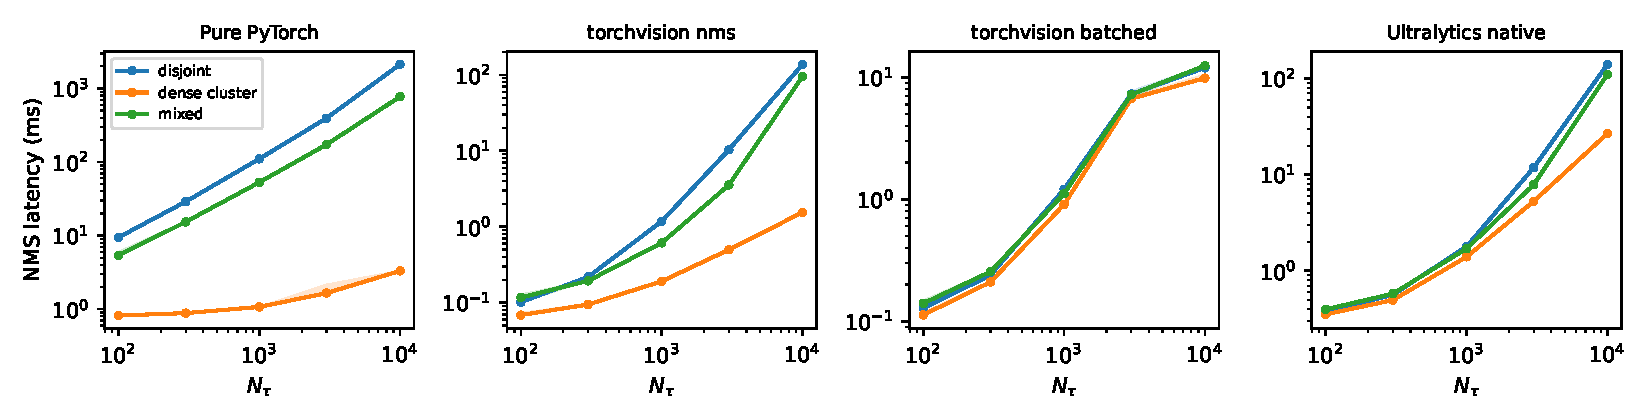
\includegraphics[width=\textwidth]{figures/fig2_dose_response.pdf}
\caption{NMS latency versus $\Ntau$ on the pinned laptop profile (grid of 10{,}000 anchors, 80 classes, no cap) for the four implementations and three box geometries. Lines are medians; shaded bands are 95\% bootstrap intervals over repetitions. Both axes are logarithmic.}
\label{fig:dose}
\end{figure*}

\subsection{Implementation, geometry, class count, and cap}
\paragraph{Implementation and geometry at equal $\Ntau$ (H2).}
At $\Ntau=300$ on the 2100-anchor head with mixed geometry, pure-PyTorch NMS is 80 times slower than torchvision \texttt{nms} (ratio 80.3, interval 76.4 to 81.9), Ultralytics-native NMS is 2.9 times slower (2.92, 2.79 to 2.98), and torchvision batched NMS 1.3 times slower (1.33, 1.24 to 1.36). Geometry matters as much as implementation. At $\Ntau=2100$, disjoint boxes take 192 times as long as dense clusters in the pure-PyTorch loop (interval 189 to 196), 13 times as long in torchvision \texttt{nms} (12.9 to 14.7), 1.8 times as long in the Ultralytics implementation (1.74 to 1.82), and no more than torchvision batched NMS (1.01, 0.89 to 1.07). At equal $\Ntau$, the cost of NMS can thus differ by more than two orders of magnitude, which is the reason that implementation and geometry are reported separately throughout.

\paragraph{Descriptive growth rates.}
Table~\ref{tab:slopes} gives the slope of the log--log curve over $\Ntau\ge100$ for the 10{,}000-anchor head. A slope near one is consistent with growth proportional to $\Ntau$ and a slope above one with faster growth, but we do not infer a complexity class from six levels; the table describes the measured curve. The dense-cluster curve of the pure-PyTorch loop is almost flat (slope 0.30), whereas torchvision \texttt{nms} on disjoint boxes grows with slope 1.59.

\begin{table}[t]
\centering\small
\caption{Log--log slope of NMS latency against $\Ntau$ over the measured levels $\ge 100$ (10{,}000-anchor head, 80 classes, no cap); 95\% bootstrap interval in brackets (all intervals are narrower than $\pm0.02$ except where shown). Descriptive only.}
\label{tab:slopes}
\begin{tabular}{@{}lccc@{}}
\toprule
Implementation & Disjoint & Dense cluster & Mixed \\
\midrule
Pure PyTorch & 1.17 [1.17, 1.17] & 0.30 [0.29, 0.32] & 1.07 [1.05, 1.08] \\
torchvision \texttt{nms} & 1.59 [1.58, 1.60] & 0.69 [0.67, 0.69] & 1.42 [1.40, 1.45] \\
torchvision batched & 1.09 [1.08, 1.10] & 1.08 [1.07, 1.09] & 1.07 [1.05, 1.08] \\
Ultralytics native & 1.29 [1.29, 1.30] & 0.96 [0.95, 0.97] & 1.21 [1.20, 1.21] \\
\bottomrule
\end{tabular}
\end{table}

\paragraph{Number of classes.}
Class-agnostic implementations are unaffected by the number of classes, as expected: at $\Ntau=2100$ with mixed geometry the median time of pure-PyTorch NMS is 114.6~ms with 80 classes and 116.5~ms with one class, and of torchvision \texttt{nms} 1.85 and 1.85~ms. The class-aware implementations are faster with one class, because boxes of different classes no longer have to be separated by the offset or the per-class loop: torchvision batched NMS takes 6.35~ms with 80 classes and 2.16~ms with one, and the Ultralytics implementation 4.45 and 2.39~ms. A class-aware detector with many classes therefore shows a different dependence on $\Ntau$ than a single-class one, and a single-class benchmark understates it.

\paragraph{Top-$k$ cap (H3).}
Table~\ref{tab:cap} shows the median NMS latency at $\Ntau=10^4$ without a cap and with a cap of 300 candidates. The cap removes most of the cost: for disjoint boxes the pure-PyTorch loop falls from 2129 to 29.6~ms, torchvision \texttt{nms} from 137 to 0.21~ms, and the Ultralytics implementation from 140 to 0.54~ms. The selection of the top 300 scores is part of the score-filter stage, which takes about 0.29~ms at $\Ntau=10^4$ without a cap and 0.39~ms with one for the pure-PyTorch arm. A deployed pipeline that caps candidates before NMS bounds the benefit that raising $\Ntau$ can bring, regardless of the optimizer.

\begin{table}[t]
\centering\small
\caption{Median NMS latency (ms) at $\Ntau=10^4$ (10{,}000-anchor head, 80 classes) without a cap and with a cap of 300 candidates.}
\label{tab:cap}
\begin{tabular}{@{}llcc@{}}
\toprule
Geometry & Implementation & No cap & Cap 300 \\
\midrule
Disjoint & Pure PyTorch & 2129 & 29.6 \\
 & torchvision \texttt{nms} & 137 & 0.210 \\
 & torchvision batched & 12.0 & 0.244 \\
 & Ultralytics native & 140 & 0.542 \\
Mixed & Pure PyTorch & 775 & 15.2 \\
 & torchvision \texttt{nms} & 95.4 & 0.184 \\
 & torchvision batched & 12.5 & 0.255 \\
 & Ultralytics native & 110 & 0.564 \\
Dense cluster & Pure PyTorch & 3.31 & 0.904 \\
 & torchvision \texttt{nms} & 1.54 & 0.102 \\
 & torchvision batched & 9.88 & 0.229 \\
 & Ultralytics native & 26.7 & 0.527 \\
\bottomrule
\end{tabular}
\end{table}

\subsection{Injection into the full pipeline (H4)}
Table~\ref{tab:pipe} reports end-to-end latency of the full pipeline for one fixed image when disjoint candidate sets are injected. With the pure-PyTorch NMS, the median time rises from 44.9~ms with no injected candidates to 303~ms at 2100, and every one of 20 repetitions exceeds the 100~ms reference deadline from 1000 candidates on. With the Ultralytics implementation the median rises only from 45.6 to 55.0~ms, and no repetition exceeds the deadline. The forward pass takes about 45~ms, so the injection moves the end-to-end time substantially only when the NMS implementation is slow enough to compete with the forward pass. The single repetition above the deadline at 100 candidates in both implementations is a timing outlier, not a dose effect: the medians at that level are 54.0 and 45.8~ms.

\begin{table}[t]
\centering\small
\caption{End-to-end latency of the full pipeline versus injected disjoint candidates (one image, 20 repetitions). Median in ms; repetitions above the 100~ms reference deadline in parentheses.}
\label{tab:pipe}
\begin{tabular}{@{}rcc@{}}
\toprule
Injected $\Ntau$ & Pure PyTorch & Ultralytics native \\
\midrule
0 & 44.9 (0) & 45.6 (0) \\
100 & 54.0 (1) & 45.8 (1) \\
300 & 75.3 (0) & 46.9 (0) \\
1000 & 154 (20) & 49.7 (0) \\
2100 & 303 (20) & 55.0 (0) \\
\bottomrule
\end{tabular}
\end{table}

\subsection{Case study: a genetic patch optimizer}
\paragraph{Optimizer.}
The case-study optimizer places a $64\times64$ overwrite patch at the window of maximum Laplacian variance of each image and evolves its pixels with a genetic algorithm (population 20, five elites, horizontal-split crossover, Gaussian mutation) under software EOT. The fitness is $\sum_i s_i \mathbb{1}[s_i>\tau]+\lambda \Ntau$ with $\lambda=1.5$, computed from pre-NMS class scores only. It contains no latency term and uses no gradients. This is the quantity whose relation to latency the study examines.
\paragraph{Scale.}
Earlier runs optimized on four images. Here the optimization set has 100 images (a fixed, seeded sample of a COCO training subset \cite{lin2014coco}), disjoint from the 100 held-out images used for measurement. Conditions are: $320$ px with a $64$ px patch ($4\%$ of the area) at $\tau=0.01$; $640$ px with a $128$ px patch (same area fraction); $320$ px with the objective threshold $\tau=0.25$; and, as a secondary condition, $640$ px with the $64$ px patch ($1\%$ of the area). Each uses ten optimization seeds and the same number of candidate evaluations as the earlier runs.
\paragraph{Baselines.}
We include random search with saliency placement, the genetic algorithm with centre placement, the genetic algorithm with random placement, and a gradient-based score-ascent baseline adapted from Overload \cite{overload2024}. The gradient baseline is an adaptation to local overwrite patches and is not a reproduction of the original.
\paragraph{Measurement.}
Patches are frozen by SHA-256 before measurement. The held-out images, with and without each patch, are measured on the pinned profile: $\Ntau$ at $\tau\in\{0.01,0.25\}$, the score-filter and NMS stages for four implementations, and end-to-end latency for two implementations.
\paragraph{Optimization outcomes on the training set.}
Table~\ref{tab:train} gives the best training fitness reached at each budget, averaged over the ten seeds. Fitness values depend on the threshold and on the input size, so they can be compared within a column group of the same input and threshold but not across groups. The genetic algorithm saturates early: for C1 the mean best fitness rises from 185.1 at 10{,}000 passes to 186.6 at 62{,}500, an increase of 0.8\%. At the final budget, random search with the same placement reaches 186.0, only 0.6 below the genetic algorithm, whereas the two placement baselines are above it (centre placement 191.0, random placement 193.5), so on this training set the placement choice moves the fitness more than the search procedure. The gradient baseline is far above all gradient-free conditions (334.1), as expected for a white-box method that uses gradients of the same objective. Wall-clock time on the GPU for one seed and the full budget is 30~s at 320 px for the gradient-free conditions, 97 to 98~s at 640 px, and 86~s for the gradient baseline.

\begin{table}[t]
\centering\small
\caption{Best training fitness (mean over ten seeds, standard deviation in parentheses) at three budgets (candidate--image forward passes).}
\label{tab:train}
\begin{tabular}{@{}lccc@{}}
\toprule
Condition & 10{,}000 & 25{,}000 & 62{,}500 \\
\midrule
C1 (320 px, $\tau_{\mathrm{obj}}$ 0.01) & 185.1 (1.7) & 185.9 (1.2) & 186.6 (1.6) \\
C3 (320 px, $\tau_{\mathrm{obj}}$ 0.25) & 39.8 (0.2) & 40.0 (0.3) & 40.5 (0.3) \\
C2 (640 px, 128 px patch) & 294.4 (3.9) & 295.5 (2.9) & 297.3 (2.2) \\
C4 (640 px, 64 px patch) & 299.4 (1.3) & 301.4 (1.9) & 303.1 (1.7) \\
B1 (centre placement) & 188.7 (1.5) & 189.8 (1.0) & 191.0 (1.4) \\
B2 (random placement) & 191.6 (1.9) & 193.1 (1.5) & 193.5 (1.9) \\
B3 (random search) & 184.5 (0.8) & 185.1 (0.8) & 186.0 (1.0) \\
B4 (gradient, tanh) & 218.1 (14.9) & 314.4 (12.8) & 334.1 (11.6) \\
\bottomrule
\end{tabular}
\end{table}

\paragraph{Results.}
The patches were generated on a GPU, frozen by hash, and measured on the pinned laptop profile (effective cores 0.84 under load; 0 of 11 reference points drift-flagged; end-to-end MDE 0.55\%). Table~\ref{tab:patches} gives ratios of patched to clean images at 320 px. Three findings stand out.

First, the genetic-algorithm patches do not raise $\Ntau$ detectably: the median $\Ntau$ at $\tau=0.01$ falls from 86.5 to 85.5 (320 px, $\tau_{\mathrm{obj}}=0.01$) and to 85 (320 px, $\tau_{\mathrm{obj}}=0.25$), and the intervals of the mean ratio include one. Random search, GA with centre placement and GA with random placement give the same picture. Second, all of them add a small but detectable amount of end-to-end time, 1.1 to 1.5\%, with intervals that exclude one but sit at about twice the end-to-end MDE; the baselines with no gradient show the same increase, so it is not specific to the optimized patches. Third, the gradient baseline raises $\Ntau$ 2.3-fold (median 93 to 166 at $\tau=0.01$; 6.7-fold at $\tau=0.25$) and raises the torchvision NMS stage by 21\% and the pure-PyTorch NMS stage 2.3-fold, but its end-to-end ratio is 1.006 with a 95\% interval of 0.997 to 1.015, which spans the MDE. Under this protocol an increase of $\Ntau$ by a factor of 2.3 is therefore not visible end to end, because on clean images NMS takes 0.16\% of the total time (median of the torchvision profile) and the forward pass dominates.

The 640-px conditions (patch of 128 px at 4\% area, and 64 px at 1\% area) raise $\Ntau$ at $\tau=0.01$ from 86.5 to 134 and from 93 to 138.5 respectively. Their time ratios against the 320-px clean images are about 3.5 to 3.6, but this is the cost of the larger input; the study design has no clean 640-px arm, so the effect of the patch at 640 px on latency is \nodata{not measured: no clean 640-px baseline} and is not interpreted.

\begin{table*}[t]
\centering\small
\caption{Effect of optimized patches relative to clean images on the pinned laptop profile. Ratios are patched over clean; intervals are 95\% two-level bootstrap intervals over images and seeds; the NMS and end-to-end columns use the torchvision pipeline; the last column is the A/A MDE of the end-to-end stage. The first three rows use 100 images $\times$ 5 seeds; the baselines use 50 images $\times$ 5 seeds.}
\label{tab:patches}
\begin{tabular}{@{}lccccc@{}}
\toprule
Condition & $\Ntau$ ratio ($\tau$=0.01) & $\Ntau$ ratio ($\tau$=0.25) & NMS latency ratio & End-to-end ratio & MDE (\%) \\
\midrule
320 px, 4\% area, $\tau$=0.01 & 1.04 (0.99--1.10) & 0.94 (0.86--1.03) & 1.003 (0.987--1.018) & 1.013 (1.006--1.021) & 0.55 \\
320 px, 4\% area, $\tau$=0.25 & 1.04 (0.99--1.09) & 0.95 (0.86--1.05) & 1.010 (0.992--1.028) & 1.015 (1.007--1.025) & 0.55 \\
640 px, 4\% area, $\tau$=0.01 & \multicolumn{5}{c}{not interpretable: no clean 640-px baseline} \\
Random search & 1.04 (0.98--1.09) & 1.00 (0.86--1.23) & 1.003 (0.981--1.028) & 1.011 (0.999--1.025) & 0.55 \\
GA, centre placement & 1.03 (0.96--1.09) & 0.92 (0.81--1.07) & 1.014 (0.991--1.037) & 1.014 (1.001--1.032) & 0.55 \\
GA, random placement & 1.05 (1.01--1.09) & 0.96 (0.89--1.04) & 1.022 (0.997--1.053) & 1.013 (1.001--1.027) & 0.55 \\
Gradient score ascent & 2.26 (1.88--2.70) & 6.7 (3.7--10.7) & 1.209 (1.170--1.248) & 1.006 (0.997--1.015) & 0.55 \\
\bottomrule
\end{tabular}
\end{table*}

\paragraph{Effect on each NMS implementation.}
Table~\ref{tab:impl} breaks the NMS-stage ratios of the 320-px conditions down by implementation. The patches from the genetic optimizer (C1, C3) and the search baselines (B1--B3) leave the NMS stage unchanged at the resolution of the protocol, with two exceptions that are within the noise of many comparisons: the pure-PyTorch ratio of C1 (1.065, interval 1.003 to 1.133) and of random placement B2 (1.071, 1.021 to 1.130) have intervals that exclude one. The gradient baseline B4 raises the NMS stage for every implementation: 2.29 for the pure-PyTorch loop, 1.21 for torchvision \texttt{nms}, and 1.11 for both class-aware implementations. At $\tau=0.25$ the pure-PyTorch and Ultralytics ratios of B4 are 4.49 and 2.50. Thus, the stage that $\Ntau$ is supposed to drive does respond to a real $\Ntau$ increase, and its response depends on the implementation, as the dose-response curves suggest.

\begin{table}[t]
\centering\small
\caption{Ratio of the NMS-stage time of patched to clean images at $\tau=0.01$ (320 px; mean ratio, 95\% two-level bootstrap interval). The A/A MDE of the NMS stage is 0.64\% for the pure-PyTorch loop and 1.1\% for torchvision \texttt{nms}.}
\label{tab:impl}
\begin{tabular}{@{}lcccc@{}}
\toprule
Condition & Pure PyTorch & \texttt{nms} & Batched & Ultralytics \\
\midrule
C1 & 1.065 (1.003--1.133) & 1.003 (0.987--1.018) & 1.000 (0.987--1.013) & 1.006 (0.991--1.023) \\
C3 & 1.059 (0.997--1.126) & 1.010 (0.992--1.028) & 1.002 (0.987--1.018) & 1.004 (0.990--1.017) \\
B1 & 1.038 (0.965--1.114) & 1.014 (0.991--1.037) & 1.000 (0.983--1.017) & 0.995 (0.978--1.013) \\
B2 & 1.071 (1.021--1.130) & 1.022 (0.997--1.053) & 1.009 (0.993--1.028) & 1.005 (0.987--1.024) \\
B3 & 1.051 (0.975--1.131) & 1.003 (0.981--1.028) & 0.995 (0.978--1.013) & 0.993 (0.974--1.013) \\
B4 & 2.285 (1.894--2.735) & 1.209 (1.170--1.248) & 1.107 (1.083--1.131) & 1.107 (1.082--1.131) \\
\bottomrule
\end{tabular}
\end{table}

\paragraph{How much of the pipeline is NMS?}
On clean images the torchvision NMS stage takes 0.16\% of the end-to-end time (median over images); the pure-PyTorch NMS stage takes 2.4\% for C1 images and 2.9\% for the images of the B4 comparison. For the gradient baseline the extra NMS time amounts to 0.034\% of the clean end-to-end time (interval 0.028\% to 0.040\%) with torchvision \texttt{nms} and to 1.9\% (1.5\% to 2.3\%) with the pure-PyTorch loop. The first is far below the end-to-end MDE of 0.55\% and the second is of the order of it, which is consistent with the end-to-end ratios of 1.006 and 1.021 reported in Table~\ref{tab:patches}. The pipeline is dominated by the forward pass, and H4 explains why: for a detector as small as YOLOv8n at 320 px, the forward pass takes about 46~ms and even a doubling of a fast NMS stage changes the total by less than the protocol can resolve.

\subsection{Does $\Ntau$ predict the latency of real candidate sets?}
For every measured unit with $\Ntau>0$ we predict $t_{\mathrm{NMS}}$ from $\Ntau$ alone by interpolating, on a log--log scale, the dose-response curve of the matching implementation and input size for each geometry. We report the median and 90th percentile of $|\ln(t_{\mathrm{measured}}/t_{\mathrm{pred}})|$ against the mixed-geometry curve and the fraction of measured points that fall between the disjoint and dense-cluster curves. These quantities describe the distance between an $\Ntau$-only prediction and the measurement; no pass/fail threshold is set in advance.
The $\Ntau$-only prediction is accurate for some implementations and poor for others. The median absolute log error against the mixed-geometry curve is 0.05 for Ultralytics-native NMS, 0.15 for torchvision batched NMS, 0.33 for torchvision \texttt{nms}, and 1.38 for pure PyTorch, i.e. a typical factor of 4 for the latter; the 90th percentiles are 0.15, 0.40, 0.47 and 1.73. The fraction of the 3347 measured points that lie between the disjoint and dense-cluster curves is 0.44, 0.35, 0.93 and 0.76 respectively. The error is about the same for clean and patched images (Table~\ref{tab:patches} arms), so the miss is a property of the synthetic curve and the real candidate sets and not of the patches. Between clean images the rank correlation of $\Ntau$ with NMS time is high (0.84 to 0.94, depending on implementation), whereas for the within-image change caused by a patch it is lower (0.36 to 0.73), which suggests that $\Ntau$ ranks images by cost better than it ranks the effect of an edit to one image. Both correlations are descriptive; the 95\% intervals are in the summary file.

\begin{figure*}[t]
\centering
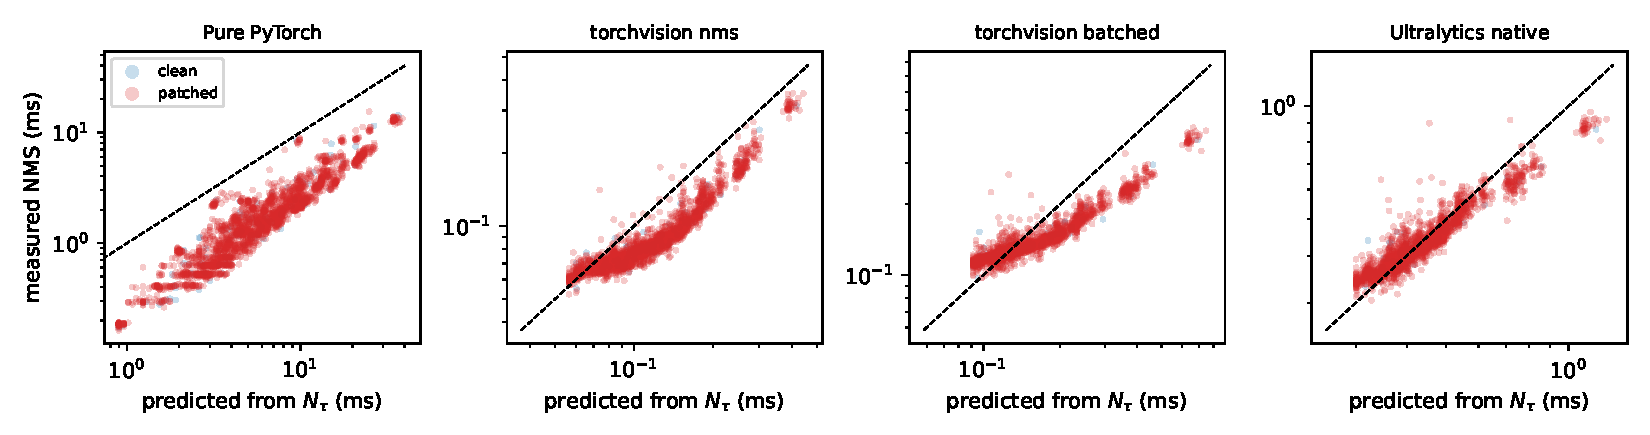
\includegraphics[width=\textwidth]{figures/fig3_pred_vs_measured.pdf}
\caption{Measured NMS latency of real candidate sets ($\tau=0.01$, 320-px conditions) versus the $\Ntau$-only prediction from the mixed-geometry dose-response curve, per implementation. The dashed line is equality. Blue points are clean images, red points are patched images (the clean points are few and mostly hidden because each clean image is a single point).}
\label{fig:pred}
\end{figure*}

\subsection{Smartphone results}
\label{sec:phone}
We planned to repeat the A/A calibration and the positive control on the smartphone. Core pinning on the device was verified under load on the fast and the slow cluster (profiles defined before the run), and no profile passed verification, so no timing was taken and no dose-response or A/A figure is reported for the smartphone. This is a negative result of the pinning protocol on this device and not a statement about its latency. Consequently the smartphone arm of the research question is not answered here; Section~\ref{sec:threats} lists it as a limitation.

\section{Discussion}
\paragraph{What the positive control establishes.}
Between $10^2$ and $10^4$ injected candidates, NMS latency grows by a factor of 4 to 1360 depending on implementation and geometry, and the growth is detected at an MDE below 1.1\%. So the number of candidates does matter for NMS time, but its effect depends on the NMS implementation and on how the boxes overlap; $\Ntau$ alone does not fix the latency. The deadline-crossing result (every repetition of the pure-PyTorch pipeline at 2100 candidates exceeds 100~ms) shows only that the test bench can produce such a miss for that implementation, not that a deployed detector would.

\paragraph{What the case study adds.}
The case-study fitness contains no latency term, so its only link to latency is the assumption that $\Ntau$ tracks it. Whether the patch effect on end-to-end latency, measured against the MDE, is consistent with what the dose-response curve predicts from the achieved $\Ntau$ is the content of Q3 and Q4. In our measurements the answer is mixed. Across images, $\Ntau$ ranks NMS time well (rank correlation above 0.84), and for the gradient baseline the pure-PyTorch NMS time rises 2.3-fold with $\Ntau$. At the level of the whole pipeline, however, the same 2.3-fold increase of $\Ntau$ changes end-to-end time by less than the interval width (1.006, interval 0.997 to 1.015), because the forward pass takes the bulk of the time at 320 px. The genetic-algorithm patches do not increase $\Ntau$ detectably, and their 1 to 1.5\% added time is shared with random search and with the baselines. We therefore find no evidence here that maximizing $\Ntau$ with this optimizer produces a latency effect, and the result for 640 px remains open because of the missing clean baseline.

\paragraph{Implications for evaluation practice.}
Reporting $\Ntau$ alone does not describe a latency effect. A latency claim needs stage-wise timing on a pinned, verified profile, an A/A estimate of the noise floor, and the NMS implementation and cap that the deployed pipeline uses. Because the cost of NMS depends on how many boxes survive, defences and attacks should be compared at equal geometry as well as equal $\Ntau$.

\paragraph{Mechanisms.}
The measurements agree with the cost model of Section~\ref{sec:results} in four respects. First, NMS latency does grow with $\Ntau$ (H1), by factors that depend on the implementation. Second, geometry decides how much (H2): the loop-based implementation spends almost all of its time on boxes that are retained, so disjoint boxes cost two orders of magnitude more than a dense cluster of the same size. Third, a cap bounds the cost (H3): at $\Ntau=10^4$ the cap of 300 reduces the pure-PyTorch time on disjoint boxes by a factor of 72 and the torchvision time by a factor of 650. Fourth, the share of NMS in the pipeline decides whether a change of the NMS stage is visible end to end (H4). What the cost model does not provide is a way to turn $\Ntau$ into milliseconds: the $\Ntau$-only prediction misses by a factor of four for the loop-based implementation, even though it is within about 5\% for the Ultralytics implementation.

\paragraph{Why the case-study optimizer does not raise $\Ntau$.}
The training fitness shows that the genetic algorithm barely improves on random search (Table~\ref{tab:train}), and that its fitness is moved more by where the patch is placed than by how its pixels are chosen. A 64-px patch covers 4\% of a 320-px image, and a score threshold of 0.01 admits all anchors with any evidence of an object, so the number of candidates is mostly determined by the image content outside the patch. A gradient method that follows the score gradient directly can raise the scores of many anchors at once and reaches 2.3 times as many candidates; a gradient-free search with 625 candidate evaluations cannot explore the space well enough. This is an observation about this optimizer and this budget and not a statement about gradient-free search in general.

\paragraph{Relation to claims in the literature.}
The reported latency increases of NMS attacks are typically obtained with a large number of boxes on a loop-based or GPU NMS kernel, on a specific edge device. Our positive control reproduces the qualitative claim in a narrow setting: with a loop-based NMS and thousands of disjoint boxes, NMS latency grows by two orders of magnitude and the end-to-end time exceeds a 100~ms reference deadline. The same control also shows how far from deployment practice this setting is: with a cap of 300 candidates the effect shrinks by one to three orders of magnitude, with a class-aware library kernel it shrinks further, and with realistic image content the number of candidates that an optimizer reaches on this detector is one to two orders of magnitude below the injected one (about 90 against $10^3$ to $10^4$). We make no claim about other detectors or devices, and we do not test the attacks that the cited works propose. Our results are consistent with the position that NMS latency attacks need a favourable combination of implementation, cap, and geometry to matter, a position that EVADE argues from a different angle \cite{evade2025}.

\paragraph{Guidance for evaluation and defence.}
For an evaluator: report $\Ntau$ together with the implementation and cap, time stages separately, report the A/A noise floor, and state which deadline is being tested and why. For a defender: a cap on the number of candidates before NMS and a library kernel with class-aware batching are the settings that make the NMS stage insensitive to $\Ntau$ in our measurements, and are cheap to adopt; the top-$k$ selection itself costs a fraction of a millisecond. For a researcher proposing a latency attack: optimize latency, or a surrogate whose relation to latency has been validated on the target pipeline, and report the effect against a noise floor.

\paragraph{What would change our conclusions.}
A larger detector in which NMS is a larger share of the pipeline, a different resolution (the real heads at 640 px have four times as many anchors), an implementation with different constant factors, or a patch optimized with a latency term instead of $\Ntau$ could produce an end-to-end effect that this study does not detect. The 640-px patch effect is left open until the clean 640-px baseline is analysed; if it is reported, it will be reported with its own noise floor.

\section{Threats to Validity}
\label{sec:threats}
This section collects the limits of the study; the results above should be read within them.
\paragraph{Internal validity.}
All laptop measurements come from one machine and one Windows power plan; the one smartphone prepared for the study failed pin verification. Timing noise is quantified with the A/A design, but the reference benchmark drifted beyond the 3\% flag in 2 of 11 blocks in the A/A run (largest change 26\%), in 2 of 12 in the positive control (largest 5.6\%) and in none of 11 in the patch re-measurement (largest 1.5\%); flagged blocks are kept in the primary analysis and the A/A has a sensitivity analysis that excludes them. The smartphone could not be pinned, so no smartphone timing exists. The patch conditions at 640 px lack a clean 640-px arm and cannot be read as latency effects. Core pinning is verified under load, but the operating system can still schedule other work on the pinned CPU. The measurement set is 100 held-out images, and patch effects use five of the ten optimization seeds. The optimization set and the measurement set are disjoint, and patches are frozen by hash before measurement. Analyses defined after inspecting data are labelled as post hoc.
\paragraph{Construct validity.}
$\Ntau$ is the number of anchors above the threshold before NMS. Latency is measured on prepared in-memory tensors, so it excludes image decoding, camera capture, and transport. The 100~ms reference deadline is a value chosen by the authors for the positive control and is not an application requirement. Synthetic candidates have controlled geometry and scores that real detections may not share, which is why the predictor is tested on real candidate sets. The pure-PyTorch NMS loop is slower than library kernels and amplifies the dependence on $\Ntau$; results are reported per implementation and not pooled.
\paragraph{External validity.}
One detector architecture (YOLOv8n, float32) and one dataset family (COCO) are studied. Two-stage detectors, NMS-free detectors such as DETR \cite{carion2020detr}, other model sizes, quantized models, and accelerators are not covered. The smartphone is an Arm SoC running Ubuntu in a proot environment on Android; it is not an embedded board, proot may add system-call overhead, and the framework builds differ from the laptop (a newer PyTorch and Ultralytics release). Had the device been pinned, we would have compared ratios and curve shapes across devices and never absolute latencies. Patches are inserted digitally with software transformations; no print-and-capture or camera evaluation was performed.
\paragraph{Conclusion validity.}
Effects are read against the A/A MDE. A confidence interval that includes one, or an effect below the MDE, is reported as not detected at that sensitivity and is not interpreted as equivalence. The patch analyses condition on the sampled images and seeds; the two-level bootstrap accounts for both sources of variation but not for other detectors or devices. Intervals are not adjusted for multiplicity because the analyses are estimates and not a family of tests.
\paragraph{Scope of the optimizer.}
The case-study optimizer is gray-box: it reads pre-NMS class scores, which a deployed service typically does not expose, and it does not minimize latency directly. The study does not claim a stronger attack than prior work, nor a denial of service in any deployed system.

\section{Conclusion}
We examined whether the number of pre-NMS candidates predicts detector latency, using a protocol that verifies core pinning under load and states the minimum detectable effect of every comparison. Between $10^2$ and $10^4$ injected candidates, NMS latency rises by a factor of 4 to 1360, depending on implementation and geometry, so the candidate count matters but does not determine latency. Genetic-algorithm patches optimized on 100 images did not raise $\Ntau$ detectably at 320 px and added 1 to 1.5\% of end-to-end time, similar to random search; a gradient baseline raised $\Ntau$ 2.3-fold without a visible end-to-end effect (interval 0.997 to 1.015, MDE 0.55\%). An $\Ntau$-only prediction of NMS time is within about 5\% for Ultralytics-native NMS but a factor of 4 off for the pure-PyTorch loop. The smartphone could not be pinned, so no Arm result is reported, and the 640-px patch effect awaits a clean 640-px baseline.

\section*{Responsible release}
The released artefacts are the measurement harness, manifests, synthetic-injection fixtures, and raw timing records. Optimized patches are not packaged as a tool, and the work is limited to a local test bench.

\section*{Data and code availability}
Code, manifests with file hashes, and raw timing records are in the project repository \url{https://github.com/reikageisme/Sponge-patch-nms}.
The repository contains the preregistration files with their version-control tags, the harness and analysis scripts, the manifests (which record the code hash, library versions, CPU topology and power plan), the hashes of every patch, the raw timing records of every run including the discarded ones, and the scripts that generate the figures. Every number in the tables can be traced to a selector in a summary file produced by a script in the repository.

\section*{Declaration of generative AI use}
An AI coding assistant (Claude Code) was used to help write and test the measurement harness and to draft parts of this manuscript. The authors specified the hypotheses and endpoints, ran the measurements, checked every reported number against the raw records, and take responsibility for the content.

\section*{Funding, acknowledgements, and competing interests}
\paragraph{Funding.} This research received no external funding; it is an independent research project of the authors.
\paragraph{Declaration of competing interests.} The authors declare no competing interests.

\bibliographystyle{unsrtnat}
\bibliography{references}

\end{document}
